\chapter{Etude terrain} % 40 pages

Lors de mon étude terrain, j'ai eu l'occasion de recenser l'avis de nombreuses personnes sur l'open source mais également sur les réflexions menée lors de mon état de l'art.

J'ai choisi d'orienter mes questionnaires et interview sur les 4 grands domaines qui représentent selon moi un pilier à améliorer, comprendre et faire évoluer pour valoriser l'open source et sur lesquel l'éditeur à la main.

Le questionnaire à été traité par une trentaine de personnes, 89\% d'entre elles ont affirmés connaitre très bien l'open source 

	\section{Plateforme promotrice}

		\subsection{Une interface pour communiquer qui laisse à désirer}

			Autour des plateformes qui contiennent et promouvoie l'open source, sur 36 personnes enregistrée, 19 indiquent qu'il y a un manque à palier dans l'interface qui permet de communiquer avec l'éditeur open source. 

			Lors de l'interview auprès de Olivier Magnial, ingénieur systèmes embarqués chez l'une des plus grande entreprise promotrice de l'open source : SMILE. Celui-ci à déclaré : 

			\begin{center}
				\textit{
				\textquote{
					Pour \gls{mainliner} du code source, un processus décrit la manière de contribuer, et c'est le plus souvent par mail.(...) Linux, par exemple c'est entièrement du mail, on à des mailing list extrêmement longues et des processus assez carrés !
				}
				}
			\end{center}

	\section{Gestion des ressources}
	\section{Chez le consommateur}

	\newpage

	\section{Marketing de l'open source}

		\subsection{L'école et l'open source}

			Une majoritée des contributeurs à l'enquête mentionne que l'on devrait bel et bien sensibiliser les gens à l'open source dans les écoles informatiques

			\begin{figure}[h]
				\center
				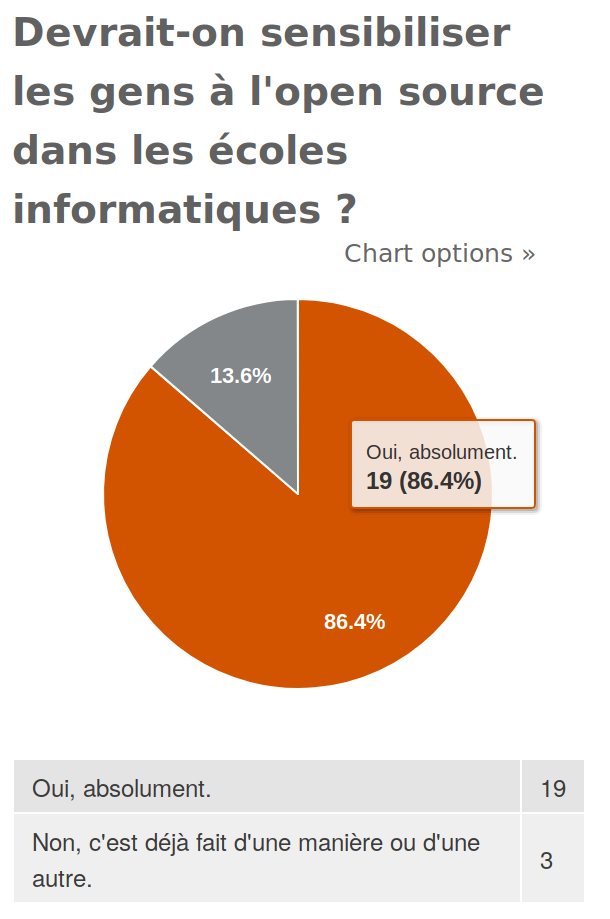
\includegraphics[scale=0.28]{./img/a6}
				\caption{Sensibiliser à l'open source}
			\end{figure}

			Plus de la moitiée des personnes, soit 21 interrogé à répondu que l'open source était peu ou tout juste assez évoqué à l'école.

			\begin{figure}[h]
				\center
				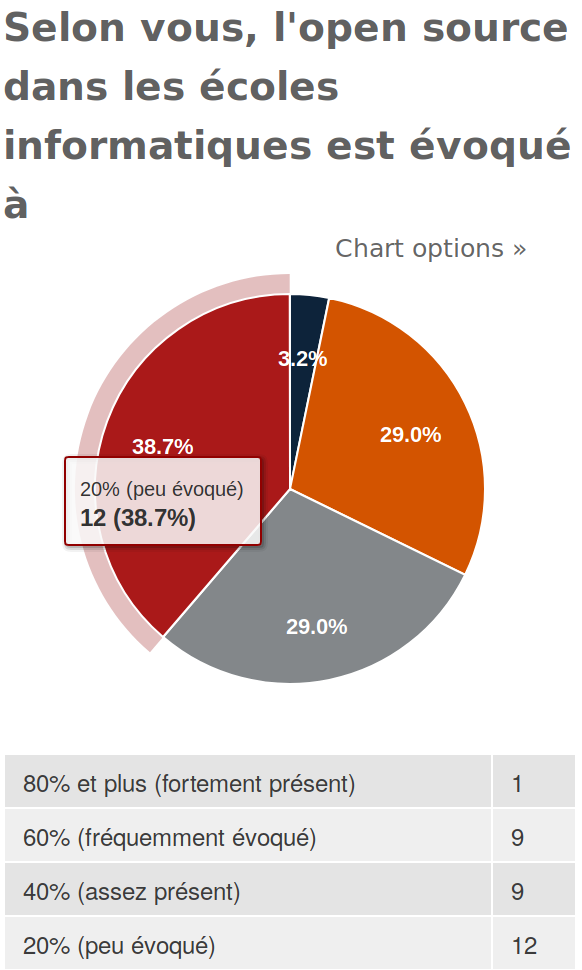
\includegraphics[scale=0.28]{./img/a5}
				\caption{L'open source à l'école}					
			\end{figure}

